\chapter{Functional Testing}
\label{chap:functional_testing}

Functional testing is a type of black-box testing that verifies the system's compliance with its specified functional requirements, as outlined in the Software Requirements Specification (SRS) document. This chapter details the functional test cases executed to ensure that each feature of the Library Management System behaves as expected from an end-user perspective, encompassing various aspects such as user interactions, data manipulations, and system responses.

The functional test cases are categorized into the following sub-sections:
\begin{itemize}
    \item Authentication and Authorization Testing
    \item Entity Management (CRUD Operations) Testing
    \item Specific Feature Testing
    \item Use Case Testing
    \item State Transition Testing
\end{itemize}

Each sub-section includes a brief overview and references the detailed test case documents located in the \`test\_artifacts/test\_cases/I\_Functional\_Testing/\` directory.

\section{Authentication and Authorization Testing}
This section focuses on verifying that user authentication (login, logout, registration) and role-based access control (RBAC) mechanisms function correctly. It ensures that only authorized users can access specific features and that security measures related to user sessions are properly enforced. The test cases cover successful logins for both Librarians and Members, various failed login scenarios, successful logouts, and verification of access restrictions for different user roles.

The detailed test cases for Authentication and Authorization are provided in:
\newpage
\documentclass[10pt, a4paper]{report}
\usepackage[utf8]{inputenc}
\usepackage{geometry}
\usepackage{longtable}
\usepackage{array} % For better column definitions in longtable
\usepackage{enumitem} % Required for itemize and enumerate options
\usepackage{helvet} % Using a sans-serif font for better readability
\renewcommand{\familydefault}{\sfdefault}

\geometry{left=0.5cm, right=0.5cm, top=2cm, bottom=2cm}

\title{Functional Test Cases: Authentication \& Authorization \\ \large Library Management System}
\author{Test Design Team (Non-Coders/Specification Experts)}
\date{May 30, 2025}

\begin{document}
\maketitle
\begin{center}
    \textbf{Note:} These test cases are designed from a black-box, user-centric perspective. Actual results and status are to be filled during test execution. Refer to the SRS for complete requirements.
\end{center}

\section*{I.A Functional Test Cases: Authentication \& Authorization}

\begin{longtable}{|>{\raggedright\arraybackslash}p{4cm}|>{\raggedright\arraybackslash}p{4cm}|>{\raggedright\arraybackslash}p{5cm}|>{\raggedright\arraybackslash}p{5cm}|}
\caption{Authentication and Authorization Test Cases}\label{tab:auth_test_cases}\\
\hline
\textbf{Test Case ID} & \textbf{Test Title} & \textbf{Test Steps} & \textbf{Expected Results} \\
\hline
\endfirsthead
\multicolumn{4}{c}%
{{\bfseries \tablename\ \thetable{} -- continued from previous page}} \\
\hline
\textbf{Test Case ID} & \textbf{Test Title} & \textbf{Test Steps} & \textbf{Expected Results} \\
\hline
\endhead
\hline \multicolumn{4}{|r|}{{Continued on next page}} \\ \hline
\endfoot
\hline
\endlastfoot

% User Registration (by Librarian)
\multicolumn{4}{|l|}{\textbf{Sub-Section: User Registration (by Librarian)}} \\ \hline
TC\_AUTH\_REG\_001 & Successful new user (Member) registration by Librarian & 
    \begin{itemize}[noitemsep, topsep=0pt, partopsep=0pt, leftmargin=*]
        \item Login as Librarian.
        \item Navigate to 'User Management' or 'Add User' section.
        \item Fill in all required fields with valid and unique data for a new 'Member' (e.g., username, password, email, full name).
        \item Submit the registration form.
    \end{itemize} & 
    \begin{itemize}[noitemsep, topsep=0pt, partopsep=0pt, leftmargin=*]
        \item System accepts the data.
        \item A success message "User registered successfully" (or similar) is displayed.
        \item The new user appears in the list of users.
        \item The new user can subsequently log in (to be tested in Login cases).
    \end{itemize} \\ \hline
TC\_AUTH\_REG\_002 & Attempt to register a new user with an existing username & 
    \begin{itemize}[noitemsep, topsep=0pt, partopsep=0pt, leftmargin=*]
        \item Login as Librarian.
        \item Navigate to 'Add User' section.
        \item Fill in user details, using a username that already exists in the system.
        \item Submit the registration form.
    \end{itemize} & 
    \begin{itemize}[noitemsep, topsep=0pt, partopsep=0pt, leftmargin=*]
        \item System rejects the registration.
        \item An appropriate error message is displayed (e.g., "Username already exists").
        \item The user is not created.
    \end{itemize} \\ \hline
TC\_AUTH\_REG\_003 & Attempt to register a new user with missing required fields & 
    \begin{itemize}[noitemsep, topsep=0pt, partopsep=0pt, leftmargin=*]
        \item Login as Librarian.
        \item Navigate to 'Add User' section.
        \item Fill in user details but leave one or more mandatory fields blank (e.g., password or email).
        \item Submit the registration form.
    \end{itemize} & 
    \begin{itemize}[noitemsep, topsep=0pt, partopsep=0pt, leftmargin=*]
        \item System rejects the registration.
        \item An appropriate error message is displayed, indicating which fields are required.
        \item The user is not created.
    \end{itemize} \\ \hline
TC\_AUTH\_REG\_004 & Attempt to register a new user with invalid data format (e.g., email) & 
    \begin{itemize}[noitemsep, topsep=0pt, partopsep=0pt, leftmargin=*]
        \item Login as Librarian.
        \item Navigate to 'Add User' section.
        \item Fill in user details, providing an incorrectly formatted email address (e.g., "usertest.com").
        \item Submit the registration form.
    \end{itemize} & 
    \begin{itemize}[noitemsep, topsep=0pt, partopsep=0pt, leftmargin=*]
        \item System rejects the registration.
        \item An appropriate error message is displayed (e.g., "Invalid email format").
        \item The user is not created.
    \end{itemize} \\ \hline

% User Login
\multicolumn{4}{|l|}{\textbf{Sub-Section: User Login}} \\ \hline
TC\_AUTH\_LOGIN\_001 & Successful login with valid Librarian credentials & 
    \begin{itemize}[noitemsep, topsep=0pt, partopsep=0pt, leftmargin=*]
        \item Navigate to the login page.
        \item Enter valid Librarian username.
        \item Enter corresponding valid password.
        \item Click the 'Login' button.
    \end{itemize} & 
    \begin{itemize}[noitemsep, topsep=0pt, partopsep=0pt, leftmargin=*]
        \item User is authenticated successfully.
        \item User is redirected to the Librarian dashboard/homepage.
        \item Librarian-specific functionalities are visible/accessible.
    \end{itemize} \\ \hline
TC\_AUTH\_LOGIN\_002 & Successful login with valid Member credentials & 
    \begin{itemize}[noitemsep, topsep=0pt, partopsep=0pt, leftmargin=*]
        \item Navigate to the login page.
        \item Enter valid Member username.
        \item Enter corresponding valid password.
        \item Click the 'Login' button.
    \end{itemize} & 
    \begin{itemize}[noitemsep, topsep=0pt, partopsep=0pt, leftmargin=*]
        \item User is authenticated successfully.
        \item User is redirected to the Member dashboard/homepage.
        \item Member-specific functionalities are visible/accessible.
    \end{itemize} \\ \hline
TC\_AUTH\_LOGIN\_003 & Attempt login with invalid username & 
    \begin{itemize}[noitemsep, topsep=0pt, partopsep=0pt, leftmargin=*]
        \item Navigate to the login page.
        \item Enter a username that does not exist.
        \item Enter any password.
        \item Click the 'Login' button.
    \end{itemize} & 
    \begin{itemize}[noitemsep, topsep=0pt, partopsep=0pt, leftmargin=*]
        \item Login fails.
        \item An appropriate error message is displayed (e.g., "Invalid username or password").
        \item User remains on the login page.
    \end{itemize} \\ \hline
TC\_AUTH\_LOGIN\_004 & Attempt login with valid username but invalid password & 
    \begin{itemize}[noitemsep, topsep=0pt, partopsep=0pt, leftmargin=*]
        \item Navigate to the login page.
        \item Enter a valid existing username.
        \item Enter an incorrect password for that username.
        \item Click the 'Login' button.
    \end{itemize} & 
    \begin{itemize}[noitemsep, topsep=0pt, partopsep=0pt, leftmargin=*]
        \item Login fails.
        \item An appropriate error message is displayed (e.g., "Invalid username or password").
        \item User remains on the login page.
    \end{itemize} \\ \hline
TC\_AUTH\_LOGIN\_005 & Attempt login with empty username field & 
    \begin{itemize}[noitemsep, topsep=0pt, partopsep=0pt, leftmargin=*]
        \item Navigate to the login page.
        \item Leave the username field empty.
        \item Enter any password.
        \item Click the 'Login' button.
    \end{itemize} & 
    \begin{itemize}[noitemsep, topsep=0pt, partopsep=0pt, leftmargin=*]
        \item Login fails.
        \item An appropriate error message is displayed (e.g., "Username is required").
        \item User remains on the login page.
    \end{itemize} \\ \hline
TC\_AUTH\_LOGIN\_006 & Attempt login with empty password field & 
    \begin{itemize}[noitemsep, topsep=0pt, partopsep=0pt, leftmargin=*]
        \item Navigate to the login page.
        \item Enter a valid username.
        \item Leave the password field empty.
        \item Click the 'Login' button.
    \end{itemize} & 
    \begin{itemize}[noitemsep, topsep=0pt, partopsep=0pt, leftmargin=*]
        \item Login fails.
        \item An appropriate error message is displayed (e.g., "Password is required").
        \item User remains on the login page.
    \end{itemize} \\ \hline

% User Logout
\multicolumn{4}{|l|}{\textbf{Sub-Section: User Logout}} \\ \hline
TC\_AUTH\_LOGOUT\_001 & Successful logout for a logged-in Librarian & 
    \begin{itemize}[noitemsep, topsep=0pt, partopsep=0pt, leftmargin=*]
        \item Login as Librarian.
        \item Click the 'Logout' button/link.
    \end{itemize} & 
    \begin{itemize}[noitemsep, topsep=0pt, partopsep=0pt, leftmargin=*]
        \item User is logged out successfully.
        \item User is redirected to the login page or public homepage.
        \item Session is terminated (user cannot access protected pages without logging in again).
    \end{itemize} \\ \hline
TC\_AUTH\_LOGOUT\_002 & Successful logout for a logged-in Member & 
    \begin{itemize}[noitemsep, topsep=0pt, partopsep=0pt, leftmargin=*]
        \item Login as Member.
        \item Click the 'Logout' button/link.
    \end{itemize} & 
    \begin{itemize}[noitemsep, topsep=0pt, partopsep=0pt, leftmargin=*]
        \item User is logged out successfully.
        \item User is redirected to the login page or public homepage.
        \item Session is terminated.
    \end{itemize} \\ \hline

% Role-Based Access Control (RBAC)
\multicolumn{4}{|l|}{\textbf{Sub-Section: Role-Based Access Control (RBAC)}} \\ \hline
TC\_AUTH\_RBAC\_001 & Verify Librarian can access Librarian-specific features (e.g., User Management) & 
    \begin{itemize}[noitemsep, topsep=0pt, partopsep=0pt, leftmargin=*]
        \item Login as Librarian.
        \item Attempt to navigate to 'User Management' section.
        \item Attempt to navigate to 'Book Management' (add/edit/delete books).
    \end{itemize} & 
    \begin{itemize}[noitemsep, topsep=0pt, partopsep=0pt, leftmargin=*]
        \item Librarian successfully accesses 'User Management' page.
        \item Librarian can view and interact with user administration tools.
        \item Librarian successfully accesses 'Book Management' page and can perform CRUD operations on books.
    \end{itemize} \\ \hline
TC\_AUTH\_RBAC\_002 & Verify Member cannot access Librarian-specific features (e.g., User Management) & 
    \begin{itemize}[noitemsep, topsep=0pt, partopsep=0pt, leftmargin=*]
        \item Login as Member.
        \item Check if 'User Management' link/button is visible.
        \item Attempt to navigate directly to the User Management URL (if known).
        \item Check if 'Add Book' or 'Edit Book' options are available.
    \end{itemize} & 
    \begin{itemize}[noitemsep, topsep=0pt, partopsep=0pt, leftmargin=*]
        \item 'User Management' link/button is not visible or is disabled.
        \item Direct navigation to User Management URL redirects to an error page or member dashboard.
        \item 'Add Book'/'Edit Book' options are not available. Access is denied.
    \end{itemize} \\ \hline
TC\_AUTH\_RBAC\_003 & Verify Member can access Member-specific features (e.g., Search Books, View Borrowal History) & 
    \begin{itemize}[noitemsep, topsep=0pt, partopsep=0pt, leftmargin=*]
        \item Login as Member.
        \item Attempt to navigate to 'Search Books' page.
        \item Attempt to view 'My Borrowal History'.
    \end{itemize} & 
    \begin{itemize}[noitemsep, topsep=0pt, partopsep=0pt, leftmargin=*]
        \item Member successfully accesses 'Search Books' page and can search.
        \item Member successfully accesses 'My Borrowal History' and can view their own history.
    \end{itemize} \\ \hline
TC\_AUTH\_RBAC\_004 & Verify guest (not logged in) user access to public pages and restriction from protected pages & 
    \begin{itemize}[noitemsep, topsep=0pt, partopsep=0pt, leftmargin=*]
        \item Ensure no user is logged in (clear session/cookies or use incognito window).
        \item Attempt to navigate to the login page.
        \item Attempt to navigate to a public book search page (if applicable).
        \item Attempt to navigate to 'User Management' URL.
        \item Attempt to navigate to 'My Borrowal History' URL.
    \end{itemize} & 
    \begin{itemize}[noitemsep, topsep=0pt, partopsep=0pt, leftmargin=*]
        \item Login page is accessible.
        \item Public book search page is accessible (if such a feature exists for guests).
        \item Access to 'User Management' URL is denied, likely redirecting to login page.
        \item Access to 'My Borrowal History' URL is denied, likely redirecting to login page.
    \end{itemize} \\ \hline

\end{longtable}

\end{document}

\section{Entity Management (CRUD Operations) Testing}
This section covers the Create, Read, Update, and Delete (CRUD) operations for the core entities of the Library Management System, including Books, Authors, Genres, Users, Borrowals, and Reviews. These tests ensure that data can be correctly managed by librarians and that members have appropriate viewing and interaction capabilities, while also verifying referential integrity constraints.

\subsection{Book Management}
Test cases for Book Management verify the addition, viewing, updating, and deletion of book records, including scenarios where deletion is prevented due to active borrowals.

\subsection{Author Management}
This covers the creation and deletion of author records, including checks for referential integrity when an author is linked to existing books.

\subsection{Genre Management}
Similar to Author Management, these test cases validate the creation and deletion of genre records, ensuring that genres linked to books cannot be deleted.

\subsection{User Management}
This sub-section tests the Librarian's ability to create, view, update, and delete user accounts (both Librarians and Members), and ensures that members cannot access user management functionalities or delete users with active borrowals.

\subsection{Borrowal Management}
Test cases for Borrowal Management verify the process of borrowing and returning books, including scenarios for borrowing unavailable books and ensuring members can only view their own borrowal history, while librarians can view all records.

\subsection{Review Management}
As a new feature, this section validates the ability of members to add reviews for books and librarians to manage (view and delete) all reviews.

The detailed test cases for Entity Management are provided in:
\documentclass[10pt, a4paper]{report}
\usepackage[utf8]{inputenc}
\usepackage{geometry}
\usepackage{longtable}
\usepackage{array} % For better column definitions in longtable
\usepackage{enumitem} % Required for itemize and enumerate options
\usepackage{helvet} % Using a sans-serif font for better readability
\renewcommand{\familydefault}{\sfdefault}

\geometry{left=1cm, right=1cm, top=2cm, bottom=2cm}

\title{Functional Test Cases: Entity Management (CRUD Operations) \\ \large Library Management System}
\author{Test Design Team (Non-Coders/Specification Experts)}
\date{June 5, 2025}

\begin{document}
\maketitle
\begin{center}
    \textbf{Note:} These test cases are designed from a black-box, user-centric perspective based on the SRS document. Actual results and status are to be filled during test execution. Test case design incorporates techniques like Equivalence Partitioning and Boundary Value Analysis.
\end{center}

\section*{I.B Functional Test Cases: Entity Management (CRUD)}

\begin{longtable}{|>{\raggedright\arraybackslash}p{4.5cm}|>{\raggedright\arraybackslash}p{4cm}|>{\raggedright\arraybackslash}p{4.5cm}|>{\raggedright\arraybackslash}p{4cm}|}
\caption{Entity Management Test Cases}\label{tab:entity_test_cases}\\
\hline
\textbf{Test Case ID} & \textbf{Test Title} & \textbf{Test Steps} & \textbf{Expected Results} \\
\hline
\endfirsthead
\multicolumn{4}{c}%
{{\bfseries \tablename\ \thetable{} -- continued from previous page}} \\
\hline
\textbf{Test Case ID} & \textbf{Test Title} & \textbf{Test Steps} & \textbf{Expected Results} \\
\hline
\endhead
\hline \multicolumn{4}{|r|}{{Continued on next page}} \\ \hline
\endfoot
\hline
\endlastfoot

% Book Management
\multicolumn{4}{|l|}{\textbf{Sub-Section: Book Management (SRS 3.3)}} \\ \hline
TC\_BOOK\_CREATE\_001 & Successful new book creation by Librarian & 
    \begin{itemize}[noitemsep, topsep=0pt, partopsep=0pt, leftmargin=*]
        \item Login as Librarian.
        \item Navigate to 'Book Management'.
        \item Click 'New Book'.
        \item Fill all required fields (Name, ISBN) with valid, unique data. Select existing Author and Genre.
        \item Submit the form.
    \end{itemize} & 
    \begin{itemize}[noitemsep, topsep=0pt, partopsep=0pt, leftmargin=*]
        \item System accepts the data.
        \item A success message is displayed.
        \item The new book appears in the book list.
    \end{itemize} \\ \hline
TC\_BOOK\_CREATE\_002 & Attempt to create a book with missing required fields & 
    \begin{itemize}[noitemsep, topsep=0pt, partopsep=0pt, leftmargin=*]
        \item Login as Librarian.
        \item Navigate to 'Book Management'.
        \item Click 'New Book'.
        \item Leave the 'Name' or 'ISBN' field blank.
        \item Submit the form.
    \end{itemize} & 
    \begin{itemize}[noitemsep, topsep=0pt, partopsep=0pt, leftmargin=*]
        \item System rejects the creation.
        \item An error message indicating required fields is displayed.
        \item The book is not created.
    \end{itemize} \\ \hline
TC\_BOOK\_CREATE\_003 & (RBAC) Verify Member cannot create a book & 
    \begin{itemize}[noitemsep, topsep=0pt, partopsep=0pt, leftmargin=*]
        \item Login as a Member.
        \item Navigate to 'Book Management'.
    \end{itemize} & 
    \begin{itemize}[noitemsep, topsep=0pt, partopsep=0pt, leftmargin=*]
        \item The 'New Book' button/option is not visible or is disabled.
        \item Direct access to the create book API endpoint (e.g., POST /api/book/add) should be denied.
    \end{itemize} \\ \hline
TC\_BOOK\_READ\_001 & Verify all users can view the list of books & 
    \begin{itemize}[noitemsep, topsep=0pt, partopsep=0pt, leftmargin=*]
        \item Login as Librarian. Navigate to 'Book Management'.
        \item Logout. Login as Member. Navigate to 'Book Management'.
    \end{itemize} & 
    \begin{itemize}[noitemsep, topsep=0pt, partopsep=0pt, leftmargin=*]
        \item Both Librarian and Member can successfully view the list of all books.
    \end{itemize} \\ \hline
TC\_BOOK\_UPDATE\_001 & Successful book update by Librarian & 
    \begin{itemize}[noitemsep, topsep=0pt, partopsep=0pt, leftmargin=*]
        \item Login as Librarian.
        \item Navigate to 'Book Management'.
        \item Select a book and choose to edit it.
        \item Modify a field (e.g., the summary).
        \item Save the changes.
    \end{itemize} & 
    \begin{itemize}[noitemsep, topsep=0pt, partopsep=0pt, leftmargin=*]
        \item System accepts the changes.
        \item A success message is displayed.
        \item The book list/details reflect the updated information.
    \end{itemize} \\ \hline
TC\_BOOK\_DELETE\_001 & Successful book deletion by Librarian & 
    \begin{itemize}[noitemsep, topsep=0pt, partopsep=0pt, leftmargin=*]
        \item Pre-condition: Create a book that has no associated borrowals.
        \item Login as Librarian.
        \item Navigate to 'Book Management'.
        \item Select the book and click 'Delete'.
        \item Confirm the deletion.
    \end{itemize} & 
    \begin{itemize}[noitemsep, topsep=0pt, partopsep=0pt, leftmargin=*]
        \item System accepts the deletion.
        \item A success message is displayed.
        \item The book is removed from the book list.
    \end{itemize} \\ \hline
TC\_BOOK\_DELETE\_002 & (Referential Integrity) Attempt to delete a book that is currently borrowed & 
    \begin{itemize}[noitemsep, topsep=0pt, partopsep=0pt, leftmargin=*]
        \item Pre-condition: A book exists and is part of an active borrowal record.
        \item Login as Librarian.
        \item Navigate to 'Book Management'.
        \item Attempt to delete the borrowed book.
    \end{itemize} & 
    \begin{itemize}[noitemsep, topsep=0pt, partopsep=0pt, leftmargin=*]
        \item System prevents the deletion.
        \item An appropriate error message is displayed (e.g., "Cannot delete a book with active borrowals").
        \item The book is not deleted.
    \end{itemize} \\ \hline

% Author Management
\multicolumn{4}{|l|}{\textbf{Sub-Section: Author Management (SRS 3.4)}} \\ \hline
TC\_AUTHOR\_CREATE\_001 & Successful new author creation by Librarian & 
    \begin{itemize}[noitemsep, topsep=0pt, partopsep=0pt, leftmargin=*]
        \item Login as Librarian.
        \item Navigate to 'Author Management'.
        \item Click 'New Author'.
        \item Fill the required 'Name' field with valid data.
        \item Submit the form.
    \end{itemize} & 
    \begin{itemize}[noitemsep, topsep=0pt, partopsep=0pt, leftmargin=*]
        \item A success message is displayed.
        \item The new author appears in the authors list.
    \end{itemize} \\ \hline
TC\_AUTHOR\_DELETE\_001 & (Referential Integrity) Attempt to delete an author linked to a book & 
    \begin{itemize}[noitemsep, topsep=0pt, partopsep=0pt, leftmargin=*]
        \item Pre-condition: An author is assigned to at least one book in the system.
        \item Login as Librarian.
        \item Navigate to 'Author Management'.
        \item Attempt to delete the author.
    \end{itemize} & 
    \begin{itemize}[noitemsep, topsep=0pt, partopsep=0pt, leftmargin=*]
        \item System prevents the deletion.
        \item An error message is displayed (e.g., "Cannot delete author assigned to existing books").
        \item The author is not deleted.
    \end{itemize} \\ \hline

% Genre Management
\multicolumn{4}{|l|}{\textbf{Sub-Section: Genre Management (SRS 3.5)}} \\ \hline
TC\_GENRE\_CREATE\_001 & Successful new genre creation by Librarian & 
    \begin{itemize}[noitemsep, topsep=0pt, partopsep=0pt, leftmargin=*]
        \item Login as Librarian.
        \item Navigate to 'Genre Management'.
        \item Click 'New Genre'.
        \item Fill the required 'Name' and 'Description' fields with valid data.
        \item Submit the form.
    \end{itemize} & 
    \begin{itemize}[noitemsep, topsep=0pt, partopsep=0pt, leftmargin=*]
        \item A success message is displayed.
        \item The new genre appears in the genres list.
    \end{itemize} \\ \hline
TC\_GENRE\_DELETE\_001 & (Referential Integrity) Attempt to delete a genre linked to a book & 
    \begin{itemize}[noitemsep, topsep=0pt, partopsep=0pt, leftmargin=*]
        \item Pre-condition: A genre is assigned to at least one book in the system.
        \item Login as Librarian.
        \item Navigate to 'Genre Management'.
        \item Attempt to delete the genre.
    \end{itemize} & 
    \begin{itemize}[noitemsep, topsep=0pt, partopsep=0pt, leftmargin=*]
        \item System prevents the deletion.
        \item An error message is displayed (e.g., "Cannot delete genre assigned to existing books").
        \item The genre is not deleted.
    \end{itemize} \\ \hline

% User Management
\multicolumn{4}{|l|}{\textbf{Sub-Section: User Management (SRS 3.7)}} \\ \hline
TC\_USER\_CREATE\_001 & Successful new user (Member) creation by Librarian & 
    \begin{itemize}[noitemsep, topsep=0pt, partopsep=0pt, leftmargin=*]
        \item Login as Librarian.
        \item Navigate to 'User Management'.
        \item Click 'New User'.
        \item Fill required fields (Name, Email, Password) with valid, unique data. Set 'isAdmin' flag to false.
        \item Submit the form.
    \end{itemize} & 
    \begin{itemize}[noitemsep, topsep=0pt, partopsep=0pt, leftmargin=*]
        \item A success message is displayed.
        \item The new user appears in the user list.
    \end{itemize} \\ \hline
TC\_USER\_CREATE\_002 & Attempt to create a user with an existing email & 
    \begin{itemize}[noitemsep, topsep=0pt, partopsep=0pt, leftmargin=*]
        \item Login as Librarian.
        \item Navigate to 'User Management'.
        \item Attempt to create a new user with an email address that is already in use.
    \end{itemize} & 
    \begin{itemize}[noitemsep, topsep=0pt, partopsep=0pt, leftmargin=*]
        \item System rejects the creation.
        \item An error message like "User already exists" is displayed.
    \end{itemize} \\ \hline
TC\_USER\_READ\_001 & (RBAC) Verify Member cannot access User Management & 
    \begin{itemize}[noitemsep, topsep=0pt, partopsep=0pt, leftmargin=*]
        \item Login as a Member.
    \end{itemize} & 
    \begin{itemize}[noitemsep, topsep=0pt, partopsep=0pt, leftmargin=*]
        \item 'User Management' link/feature is not visible or is disabled.
        \item Direct navigation to the user management URL is denied.
    \end{itemize} \\ \hline
TC\_USER\_DELETE\_001 & (Referential Integrity) Attempt to delete a member with active borrowals & 
    \begin{itemize}[noitemsep, topsep=0pt, partopsep=0pt, leftmargin=*]
        \item Pre-condition: A member has one or more active (not returned) borrowal records.
        \item Login as Librarian.
        \item Navigate to 'User Management'.
        \item Attempt to delete the member.
    \end{itemize} & 
    \begin{itemize}[noitemsep, topsep=0pt, partopsep=0pt, leftmargin=*]
        \item System prevents the deletion.
        \item An error message is displayed (e.g., "Cannot delete member with active borrowals").
        \item The user is not deleted.
    \end{itemize} \\ \hline

% Borrowal Management
\multicolumn{4}{|l|}{\textbf{Sub-Section: Borrowal Management (SRS 3.6)}} \\ \hline
TC\_BORROW\_CREATE\_001 & Successful borrowal creation by Member & 
    \begin{itemize}[noitemsep, topsep=0pt, partopsep=0pt, leftmargin=*]
        \item Pre-condition: A book is available (isAvailable=true).
        \item Login as Member.
        \item Navigate to 'Borrowal Management'.
        \item Click 'New Borrowal' and select an available book.
        \item Submit the form.
    \end{itemize} & 
    \begin{itemize}[noitemsep, topsep=0pt, partopsep=0pt, leftmargin=*]
        \item A new borrowal record is created with 'Borrowed' status.
        \item A success message is displayed.
        \item The book's availability status is updated to 'false'.
    \end{itemize} \\ \hline
TC\_BORROW\_CREATE\_002 & Attempt to borrow an unavailable book & 
    \begin{itemize}[noitemsep, topsep=0pt, partopsep=0pt, leftmargin=*]
        \item Pre-condition: A book is unavailable (isAvailable=false).
        \item Login as Member.
        \item Attempt to create a borrowal for the unavailable book.
    \end{itemize} & 
    \begin{itemize}[noitemsep, topsep=0pt, partopsep=0pt, leftmargin=*]
        \item The system prevents the borrowal.
        \item An appropriate error message is displayed (e.g., "Book is not available").
    \end{itemize} \\ \hline
TC\_BORROW\_READ\_001 & Verify Member can only see their own borrowal history & 
    \begin{itemize}[noitemsep, topsep=0pt, partopsep=0pt, leftmargin=*]
        \item Pre-condition: Multiple members have borrowal records.
        \item Login as Member 1.
        \item Navigate to 'Borrowal Management'.
    \end{itemize} & 
    \begin{itemize}[noitemsep, topsep=0pt, partopsep=0pt, leftmargin=*]
        \item The list only displays borrowals where the memberId matches Member 1's ID.
        \item Borrowals for other members are not visible.
    \end{itemize} \\ \hline
TC\_BORROW\_UPDATE\_001 & Successful borrowal update by Librarian (mark as returned) & 
    \begin{itemize}[noitemsep, topsep=0pt, partopsep=0pt, leftmargin=*]
        \item Pre-condition: An active borrowal exists.
        \item Login as Librarian.
        \item Navigate to 'Borrowal Management'.
        \item Select the active borrowal and edit it.
        \item Change the status to 'Returned'.
        \item Save the changes.
    \end{itemize} & 
    \begin{itemize}[noitemsep, topsep=0pt, partopsep=0pt, leftmargin=*]
        \item The borrowal record status is updated.
        \item The associated book's 'isAvailable' status should ideally be updated to 'true'.
        \item A success message is displayed.
    \end{itemize} \\ \hline

% Review Management
\multicolumn{4}{|l|}{\textbf{Sub-Section: Review Management (SRS 3.8)}} \\ \hline
TC\_REVIEW\_CREATE\_001 & (Assumed) Successful review creation by Member & 
    \begin{itemize}[noitemsep, topsep=0pt, partopsep=0pt, leftmargin=*]
        \item Pre-condition: Based on assumed member capabilities if UI were present.
        \item Login as Member.
        \item Navigate to a specific book's detail page.
        \item Submit a new review with a star rating and text.
    \end{itemize} & 
    \begin{itemize}[noitemsep, topsep=0pt, partopsep=0pt, leftmargin=*]
        \item A success message is displayed.
        \item The new review is visible on the book's page.
    \end{itemize} \\ \hline
TC\_REVIEW\_CREATE\_002 & Attempt to create a review with invalid data & 
    \begin{itemize}[noitemsep, topsep=0pt, partopsep=0pt, leftmargin=*]
        \item Login as Member.
        \item Attempt to submit a review with a required field missing (e.g., star rating) or an invalid value (e.g., 6 stars).
    \end{itemize} & 
    \begin{itemize}[noitemsep, topsep=0pt, partopsep=0pt, leftmargin=*]
        \item System rejects the submission.
        \item An appropriate error message is displayed.
    \end{itemize} \\ \hline
TC\_REVIEW\_DELETE\_001 & Successful review deletion by Librarian & 
    \begin{itemize}[noitemsep, topsep=0pt, partopsep=0pt, leftmargin=*]
        \item Pre-condition: A review exists for a book.
        \item Login as Librarian.
        \item Navigate to the book or a review management section.
        \item Select a review and delete it.
    \end{itemize} & 
    \begin{itemize}[noitemsep, topsep=0pt, partopsep=0pt, leftmargin=*]
        \item The review is successfully deleted.
        \item The review is no longer visible.
    \end{itemize} \\ \hline

\multicolumn{4}{|l|}{\textbf{Entity: Review Management (new feat)}} \\ \hline
TC\_REVIEW\_CREATE\_001 \& Successful review creation by Member (new feat) & 
	\begin{itemize}[noitemsep, topsep=0pt, partopsep=0pt, leftmargin=*]
		\item Login as Member.
		\item Navigate to a specific book's detail page.
		\item Submit a new review with a star rating and text.
	\end{itemize} & 
	\begin{itemize}[noitemsep, topsep=0pt, partopsep=0pt, leftmargin=*]
		\item A success message is displayed.
		\item The new review is visible on the book's page.
	\end{itemize} \\ \hline
TC\_REVIEW\_CREATE\_002 & Attempt to create a review with invalid data (new feat) & 
	\begin{itemize}[noitemsep, topsep=0pt, partopsep=0pt, leftmargin=*]
		\item Login as Member.
		\item Attempt to submit a review with a required field missing (e.g., star rating) or an invalid value (e.g., 6 stars).
	\end{itemize} & 
	\begin{itemize}[noitemsep, topsep=0pt, partopsep=0pt, leftmargin=*]
		\item System rejects the submission.
		\item An appropriate error message is displayed.
	\end{itemize} \\ \hline
TC\_REVIEW\_DELETE\_001 & Successful review deletion by Librarian (new feat) & 
	\begin{itemize}[noitemsep, topsep=0pt, partopsep=0pt, leftmargin=*]
		\item Pre-condition: A review exists for a book.
		\item Login as Librarian.
		\item Navigate to the book or a review management section.
		\item Select a review and delete it.
	\end{itemize} & 
	\begin{itemize}[noitemsep, topsep=0pt, partopsep=0pt, leftmargin=*]
		\item The review is removed from the system.
		\item A success confirmation message is shown.
	\end{itemize} \\ \hline

\end{longtable}

\end{document}

\section{Specific Feature Testing}
This section focuses on testing specific functionalities within the system that might not be fully covered by CRUD or Use Case tests, such as the Librarian Dashboard and detailed access controls for various entities. These tests ensure that individual features operate as designed and that role-based permissions are respected.

\subsection{Dashboard (Librarian)}
Verifies that only Librarians can access the dashboard and that it displays relevant overview statistics and charts.

\begin{figure}[H]
    \centering
    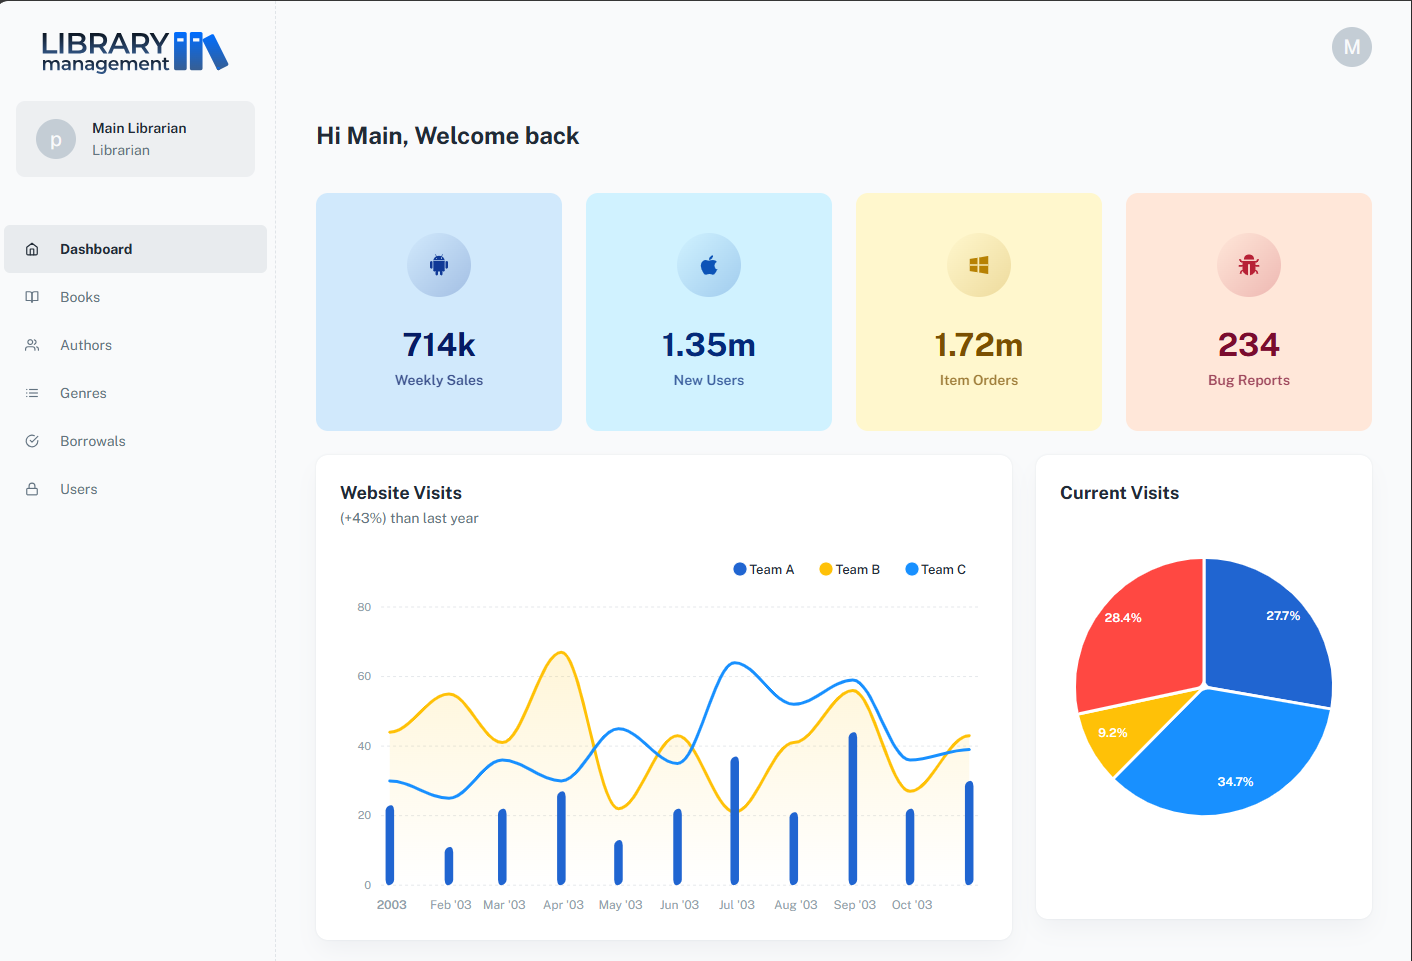
\includegraphics[width=0.8\textwidth]{assets/dashboard_screenshot.png} % Placeholder for Dashboard Screenshot
    \caption{Librarian Dashboard Overview}
    \label{fig:dashboard_overview}
\end{figure}

\subsection{Book Management (Detailed)}
Further tests on book CRUD operations, particularly focusing on UI element visibility and direct API access denial for members.

\subsection{Borrowal Management (Detailed)}
Additional tests to confirm successful borrowal requests, handling of unavailable books, and verification of role-based viewing of borrowal history.

\subsection{User Management (by Librarian) (Detailed)}
Detailed tests for Librarian's abilities to manage user accounts, including viewing all users, updating details, and successful deletion.

\subsection{Review Management (Detailed)}
Detailed tests on the new review feature, including addition and deletion by appropriate roles, and general visibility of reviews.

The detailed test cases for Specific Feature Testing are provided in:
\documentclass[10pt, a4paper]{report}
\usepackage[utf8]{inputenc}
\usepackage{geometry}
\usepackage{longtable}
\usepackage{array} % For better column definitions in longtable
\usepackage{enumitem} % Required for itemize and enumerate options
\usepackage{helvet} % Using a sans-serif font for better readability
\renewcommand{\familydefault}{\sfdefault}

\geometry{left=1cm, right=1cm, top=2cm, bottom=2cm}

\title{Functional Test Cases: Specific Feature Testing \\ \large Library Management System}
\author{Test Design Team (Non-Coders/Specification Experts)}
\date{June 5, 2025}

\begin{document}
\maketitle
\begin{center}
    \textbf{Note:} These test cases are designed from a black-box, user-centric perspective based on the SRS document. Actual results and status are to be filled during test execution.
\end{center}

\section*{I.C Functional Test Cases: Specific Feature Testing}

\begin{longtable}{|>{\raggedright\arraybackslash}p{3.5cm}|>{\raggedright\arraybackslash}p{4.5cm}|>{\raggedright\arraybackslash}p{4.5cm}|>{\raggedright\arraybackslash}p{4.5cm}|}
\caption{Specific Feature Test Cases}\label{tab:feature_test_cases}\\
\hline
\textbf{Test Case ID} & \textbf{Test Title} & \textbf{Test Steps} & \textbf{Expected Results} \\
\hline
\endfirsthead
\multicolumn{4}{c}%
{{\bfseries \tablename\ \thetable{} -- continued from previous page}} \\
\hline
\textbf{Test Case ID} & \textbf{Test Title} & \textbf{Test Steps} & \textbf{Expected Results} \\
\hline
\endhead
\hline \multicolumn{4}{|r|}{{Continued on next page}} \\ \hline
\endfoot
\hline
\endlastfoot

% Sub-Section: Dashboard (Librarian)
\multicolumn{4}{|l|}{\textbf{Sub-Section: Dashboard (Librarian)}} \\ \hline
TC\_DASH\_001 & Verify Librarian can access the Dashboard & 
    \begin{itemize}[noitemsep, topsep=0pt, partopsep=0pt, leftmargin=*]
        \item Login as Librarian.
        \item Navigate to the Dashboard.
    \end{itemize} & 
    \begin{itemize}[noitemsep, topsep=0pt, partopsep=0pt, leftmargin=*]
        \item User is successfully redirected to the Librarian dashboard at '/dashboard'.
        \item Dashboard displays overview statistics and charts.
    \end{itemize} \\ \hline
TC\_DASH\_002 & Verify Member cannot access the Dashboard & 
    \begin{itemize}[noitemsep, topsep=0pt, partopsep=0pt, leftmargin=*]
        \item Login as a 'Member' user.
        \item Attempt to navigate directly to the '/dashboard' URL.
    \end{itemize} & 
    \begin{itemize}[noitemsep, topsep=0pt, partopsep=0pt, leftmargin=*]
        \item Access is denied.
        \item User is redirected to the member landing page (e.g., '/books') or an error page.
    \end{itemize} \\ \hline

% Sub-Section: Book Management (CRUD)
\multicolumn{4}{|l|}{\textbf{Sub-Section: Book Management (CRUD)}} \\ \hline
TC\_BOOK\_ADD\_001 & Successful new book creation by Librarian &
    \begin{itemize}[noitemsep, topsep=0pt, partopsep=0pt, leftmargin=*]
        \item Login as Librarian.
        \item Navigate to 'Book Management' (/books).
        \item Click "New Book" button.
        \item Fill in all required fields (Name, ISBN) with valid data.
        \item Select existing Author and Genre.
        \item Submit the form.
    \end{itemize} &
    \begin{itemize}[noitemsep, topsep=0pt, partopsep=0pt, leftmargin=*]
        \item A success message is displayed.
        \item The new book record is created and appears in the book list.
    \end{itemize} \\ \hline
TC\_BOOK\_ADD\_002 & Attempt to create a book with missing required fields &
    \begin{itemize}[noitemsep, topsep=0pt, partopsep=0pt, leftmargin=*]
        \item Login as Librarian.
        \item Navigate to 'Book Management'.
        \item Open the "Add Book" form.
        \item Leave a required field (e.g., Name) blank.
        \item Submit the form.
    \end{itemize} &
    \begin{itemize}[noitemsep, topsep=0pt, partopsep=0pt, leftmargin=*]
        \item The system rejects the submission.
        \item An error message indicating the required field is missing is displayed.
        \item The book is not added to the database.
    \end{itemize} \\ \hline
TC\_BOOK\_VIEW\_001 & Verify Member can view list of books and book details &
    \begin{itemize}[noitemsep, topsep=0pt, partopsep=0pt, leftmargin=*]
        \item Login as Member.
        \item Navigate to 'Book Management' (/books).
        \item Click on a specific book in the list.
    \end{itemize} &
    \begin{itemize}[noitemsep, topsep=0pt, partopsep=0pt, leftmargin=*]
        \item Member can successfully view the list of all books.
        \item Member can successfully view the details of a specific book.
    \end{itemize} \\ \hline
TC\_BOOK\_UPD\_001 & Successful update of a book's details by Librarian &
    \begin{itemize}[noitemsep, topsep=0pt, partopsep=0pt, leftmargin=*]
        \item Login as Librarian.
        \item Navigate to 'Book Management'.
        \item Select a book to edit.
        \item Change a field (e.g., update the summary).
        \item Save the changes.
    \end{itemize} &
    \begin{itemize}[noitemsep, topsep=0pt, partopsep=0pt, leftmargin=*]
        \item A success message is displayed.
        \item The updated information is reflected correctly in the book's detail view.
    \end{itemize} \\ \hline
TC\_BOOK\_DEL\_001 & Successful deletion of a book by Librarian &
    \begin{itemize}[noitemsep, topsep=0pt, partopsep=0pt, leftmargin=*]
        \item Login as Librarian.
        \item Navigate to 'Book Management'.
        \item Select a book to delete.
        \item Confirm the deletion in the dialog.
    \end{itemize} &
    \begin{itemize}[noitemsep, topsep=0pt, partopsep=0pt, leftmargin=*]
        \item A success message is displayed.
        \item The book is removed from the book list.
    \end{itemize} \\ \hline
TC\_BOOK\_ACCESS\_001 & Verify Member cannot access book CRUD operations &
    \begin{itemize}[noitemsep, topsep=0pt, partopsep=0pt, leftmargin=*]
        \item Login as Member.
        \item Navigate to 'Book Management'.
    \end{itemize} &
    \begin{itemize}[noitemsep, topsep=0pt, partopsep=0pt, leftmargin=*]
        \item "Add Book", "Edit Book", and "Delete Book" UI elements are not visible or are disabled.
        \item Direct access to corresponding API endpoints is denied.
    \end{itemize} \\ \hline
    
% Sub-Section: Borrowal Management
\multicolumn{4}{|l|}{\textbf{Sub-Section: Borrowal Management}} \\ \hline
TC\_BORW\_ADD\_001 & Successful borrowal request by Member for an available book &
    \begin{itemize}[noitemsep, topsep=0pt, partopsep=0pt, leftmargin=*]
        \item Login as Member.
        \item Navigate to 'Borrowal Management' (/borrowals).
        \item Click "New Borrowal".
        \item Select a book that is marked as available.
        \item Submit the form.
    \end{itemize} &
    \begin{itemize}[noitemsep, topsep=0pt, partopsep=0pt, leftmargin=*]
        \item A success message is displayed.
        \item A new borrowal record is created with 'Borrowed' status and correct dates.
        \item The new record appears in the member's borrowal history.
    \end{itemize} \\ \hline
TC\_BORW\_ADD\_002 & Attempt to borrow a book that is not available &
    \begin{itemize}[noitemsep, topsep=0pt, partopsep=0pt, leftmargin=*]
        \item Login as Member.
        \item Navigate to 'Borrowal Management'.
        \item Attempt to create a new borrowal for a book that is not available.
    \end{itemize} &
    \begin{itemize}[noitemsep, topsep=0pt, partopsep=0pt, leftmargin=*]
        \item The UI should clearly indicate the book is not available.
        \item The system prevents the submission or displays a clear error message.
    \end{itemize} \\ \hline
TC\_BORW\_VIEW\_001 & Verify Member can only view their own borrowal history &
    \begin{itemize}[noitemsep, topsep=0pt, partopsep=0pt, leftmargin=*]
        \item Login as a Member who has borrowal records.
        \item Navigate to 'Borrowal Management' (/borrowals).
    \end{itemize} &
    \begin{itemize}[noitemsep, topsep=0pt, partopsep=0pt, leftmargin=*]
        \item The list displays only the borrowals associated with the logged-in member's ID.
        \item Records of other members are not visible.
    \end{itemize} \\ \hline
TC\_BORW\_VIEW\_002 & Verify Librarian can view all borrowal records &
    \begin{itemize}[noitemsep, topsep=0pt, partopsep=0pt, leftmargin=*]
        \item Login as Librarian.
        \item Navigate to 'Borrowal Management'.
    \end{itemize} &
    \begin{itemize}[noitemsep, topsep=0pt, partopsep=0pt, leftmargin=*]
        \item A list of all borrowal records for all members is displayed.
    \end{itemize} \\ \hline
TC\_BORW\_UPD\_001 & Successful update of borrowal status by Librarian &
    \begin{itemize}[noitemsep, topsep=0pt, partopsep=0pt, leftmargin=*]
        \item Login as Librarian.
        \item Navigate to 'Borrowal Management'.
        \item Select an existing 'Borrowed' record.
        \item Update its status to 'Returned'.
        \item Save the change.
    \end{itemize} &
    \begin{itemize}[noitemsep, topsep=0pt, partopsep=0pt, leftmargin=*]
        \item A success message is displayed.
        \item The record's status is correctly updated in the list.
    \end{itemize} \\ \hline
    
% Sub-Section: User Management (by Librarian)
\multicolumn{4}{|l|}{\textbf{Sub-Section: User Management (by Librarian)}} \\ \hline
TC\_USER\_VIEW\_001 & Verify Librarian can view list of all users &
    \begin{itemize}[noitemsep, topsep=0pt, partopsep=0pt, leftmargin=*]
        \item Login as Librarian.
        \item Navigate to 'User Management' (/users).
    \end{itemize} &
    \begin{itemize}[noitemsep, topsep=0pt, partopsep=0pt, leftmargin=*]
        \item A list of all users (both Librarians and Members) is displayed correctly.
    \end{itemize} \\ \hline
TC\_USER\_UPD\_001 & Successful update of a user's details by Librarian &
    \begin{itemize}[noitemsep, topsep=0pt, partopsep=0pt, leftmargin=*]
        \item Login as Librarian.
        \item Navigate to 'User Management'.
        \item Select a user to edit.
        \item Update a non-critical field (e.g., Phone number).
        \item Save the changes.
    \end{itemize} &
    \begin{itemize}[noitemsep, topsep=0pt, partopsep=0pt, leftmargin=*]
        \item A success message is displayed.
        \item The user's details are correctly updated.
    \end{itemize} \\ \hline
TC\_USER\_DEL\_001 & Successful deletion of a user by Librarian &
    \begin{itemize}[noitemsep, topsep=0pt, partopsep=0pt, leftmargin=*]
        \item Login as Librarian.
        \item Navigate to 'User Management'.
        \item Select a user account to delete.
        \item Confirm the deletion.
    \end{itemize} &
    \begin{itemize}[noitemsep, topsep=0pt, partopsep=0pt, leftmargin=*]
        \item A success message is displayed.
        \item The user is removed from the list of users.
        \item The deleted user can no longer log in.
    \end{itemize} \\ \hline

% Sub-Section: Review Management
\multicolumn{4}{|l|}{\textbf{Sub-Section: Review Management (Assumed Admin UI)}} \\ \hline
TC\_REV\_ADD\_001 & Successful addition of a review by Librarian (Admin action) &
    \begin{itemize}[noitemsep, topsep=0pt, partopsep=0pt, leftmargin=*]
        \item Login as Librarian.
        \item Navigate to a book's detail page.
        \item Use an administrative function to add a review for the book.
        \item Enter a star rating and review text.
        \item Submit the review.
    \end{itemize} &
    \begin{itemize}[noitemsep, topsep=0pt, partopsep=0pt, leftmargin=*]
        \item A success message is displayed.
        \item The new review appears in the list of reviews for that book.
    \end{itemize} \\ \hline
TC\_REV\_VIEW\_001 & Verify any user can view reviews for a book &
    \begin{itemize}[noitemsep, topsep=0pt, partopsep=0pt, leftmargin=*]
        \item As any logged-in user (or guest, if public).
        \item Navigate to the detail page of a book that has reviews.
    \end{itemize} &
    \begin{itemize}[noitemsep, topsep=0pt, partopsep=0pt, leftmargin=*]
        \item The list of reviews for the book is displayed correctly.
    \end{itemize} \\ \hline
TC\_REV\_DEL\_001 & Successful deletion of a review by Librarian &
    \begin{itemize}[noitemsep, topsep=0pt, partopsep=0pt, leftmargin=*]
        \item Login as Librarian.
        \item Navigate to a book with reviews.
        \item Select a specific review to delete.
        \item Confirm the deletion.
    \end{itemize} &
    \begin{itemize}[noitemsep, topsep=0pt, partopsep=0pt, leftmargin=*]
        \item A success message is displayed.
        \item The review is removed from the book's list of reviews.
    \end{itemize} \\ \hline

\end{longtable}

\end{document}

\section{Use Case Testing}
Use Case testing directly validates the main and alternative flows of key user interactions as defined in the SRS's Use Case section. This approach ensures that the system supports essential user tasks comprehensively.

\subsection{UC-002: Add New Book (Librarian)}
Verifies the complete process of a Librarian adding a new book, including successful scenarios and handling of missing required fields or backend validation failures.

\subsection{UC-003: Borrow a Book (Member)}
Ensures that members can successfully borrow available books, that the system prevents borrowing unavailable books, and that the borrowal form correctly auto-populates relevant data.

\subsection{UC-005: View Borrowal History (Member)}
Validates a member's ability to view their own borrowal history, including scenarios with empty history and ensuring proper role-based viewing (members see only theirs, librarians see all).

\begin{figure}[H]
    \centering
    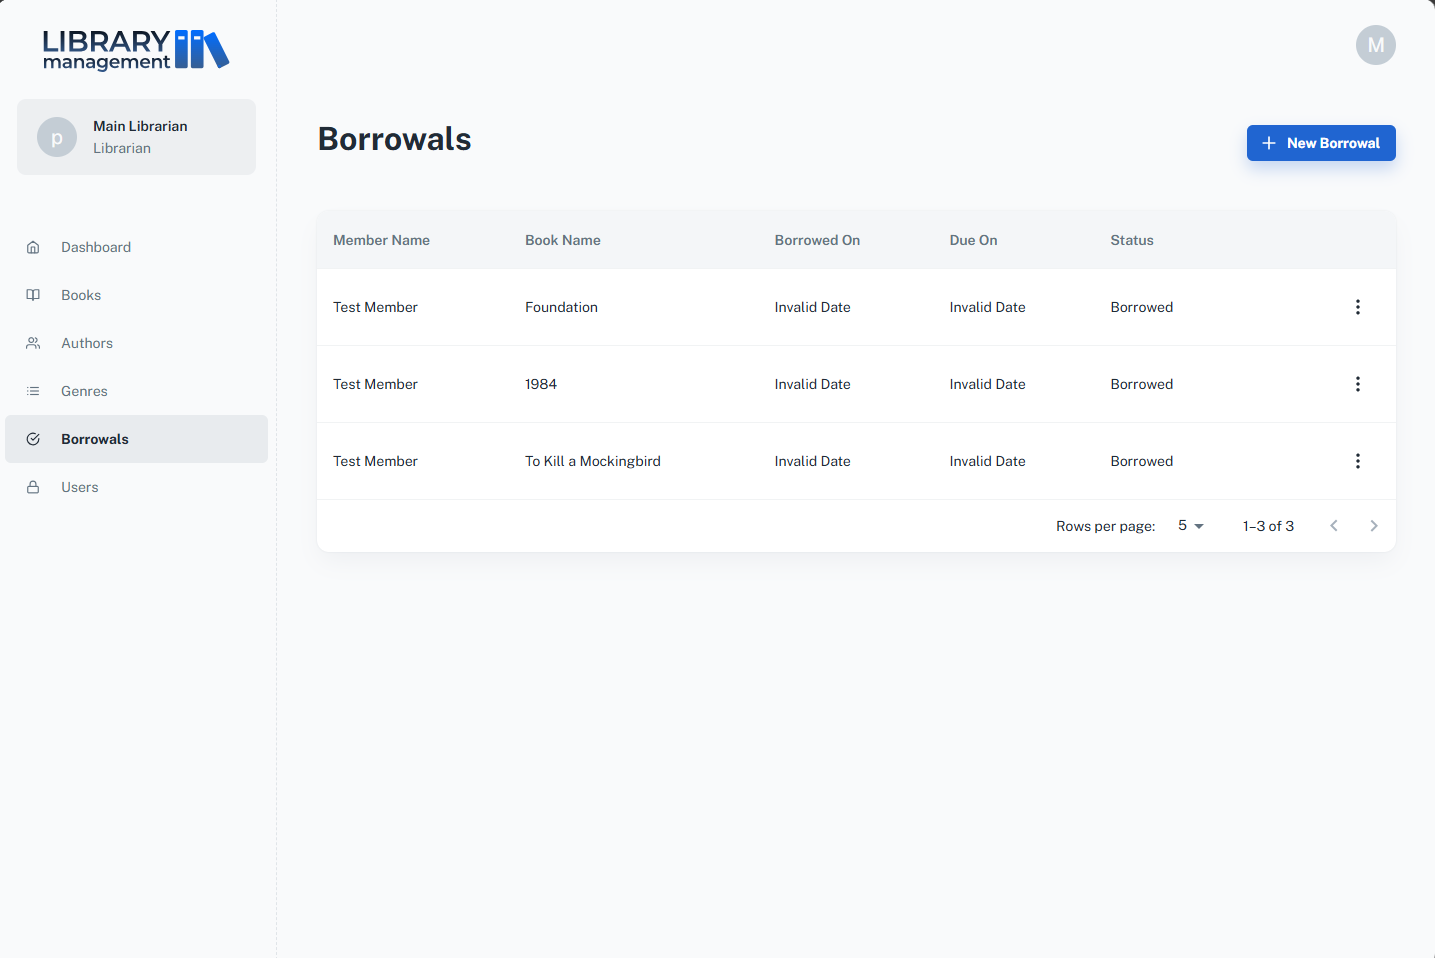
\includegraphics[width=0.8\textwidth]{assets/borrowal_history_member.png} % Placeholder for Member Borrowal History Screenshot
    \caption{Member's Borrowal History View}
    \label{fig:borrowal_history_member}
\end{figure}

The detailed test cases for Use Case Testing are provided in:
\begin{longtable}{|>{\scriptsize\raggedright\arraybackslash}p{3.5cm}|>{\raggedright\arraybackslash}p{3.5cm}|>{\raggedright\arraybackslash}p{4cm}|>{\raggedright\arraybackslash}p{4cm}|}
\caption{Use Case Test Cases}\label{tab:use_case_tests}\\
\hline
\textbf{Test Case ID} & \textbf{Test Title / Use Case} & \textbf{Test Steps} & \textbf{Expected Results} \\
\hline
\endfirsthead
\multicolumn{4}{c}%
{{\bfseries \tablename\ \thetable{} -- continued from previous page}} \\
\hline
\textbf{Test Case ID} & \textbf{Test Title / Use Case} & \textbf{Test Steps} & \textbf{Expected Results} \\
\hline
\endhead
\hline \multicolumn{4}{|r|}{{Continued on next page}} \\ \hline
\endfoot
\hline
\endlastfoot

% UC-002: Add New Book (Librarian)
\multicolumn{4}{|l|}{\textbf{Sub-Section: UC-002: Add New Book (Librarian) }} \\ \hline
TC\_UC\_BOOK\_001 & Successful addition of a new book (Main Flow) & 
    \begin{itemize}[noitemsep, topsep=0pt, partopsep=0pt, leftmargin=*]
        \item As a logged-in Librarian, navigate to the Book Management page (`/books`).
        \item Click the "New Book" button.
        \item Fill in all required fields (Name, ISBN) with valid data.
        \item Select a valid Author and Genre from the provided lists.
        \item Ensure "Is Available" is set to true.
        \item Submit the form.
    \end{itemize} & 
    \begin{itemize}[noitemsep, topsep=0pt, partopsep=0pt, leftmargin=*]
        \item The system creates a new book record via `POST /api/book/add`.
        \item A success message is displayed (e.g., "Book added").
        \item The "Add Book" form closes.
        \item The new book appears in the list on the Book Management page.
    \end{itemize} \\ \hline
TC\_UC\_BOOK\_002 & Attempt to add a book with missing required fields (Alternative Flow A1) & 
    \begin{itemize}[noitemsep, topsep=0pt, partopsep=0pt, leftmargin=*]
        \item As a logged-in Librarian, navigate to the "Add Book" form.
        \item Fill in the form but leave a required field (e.g., Name) blank.
        \item Submit the form.
    \end{itemize} & 
    \begin{itemize}[noitemsep, topsep=0pt, partopsep=0pt, leftmargin=*]
        \item The system rejects the submission due to a validation error.
        \item An error message is displayed, indicating the required field is missing.
        \item The form remains open for correction.
        \item The book is not added to the database.
    \end{itemize} \\ \hline
TC\_UC\_BOOK\_003 & Attempt to add a book that fails backend validation (Alternative Flow A2) & 
    \begin{itemize}[noitemsep, topsep=0pt, partopsep=0pt, leftmargin=*]
        \item As a logged-in Librarian, navigate to the "Add Book" form.
        \item Fill in all fields with data that is syntactically valid on the client-side but might trigger a server error (e.g., a duplicate ISBN if the server enforces uniqueness).
        \item Submit the form.
    \end{itemize} & 
    \begin{itemize}[noitemsep, topsep=0pt, partopsep=0pt, leftmargin=*]
        \item The system displays a generic error message from the API (e.g., "Something went wrong, please try again").
        \item The book is not added to the database.
    \end{itemize} \\ \hline

% UC-003: Borrow a Book (Member)
\multicolumn{4}{|l|}{\textbf{Sub-Section: UC-003: Borrow a Book (Member) }} \\ \hline
TC\_UC\_BORROW\_001 & Successful borrowing of an available book (Main Flow) & 
    \begin{itemize}[noitemsep, topsep=0pt, partopsep=0pt, leftmargin=*]
        \item As a logged-in Member, navigate to the Borrowal Management page (`/borrowals`).
        \item Click the "New Borrowal" button.
        \item Select a book that is marked as available from the list.
        \item Verify that the Member field is correctly auto-populated.
        \item Submit the form.
    \end{itemize} & 
    \begin{itemize}[noitemsep, topsep=0pt, partopsep=0pt, leftmargin=*]
        \item A new borrowal record is created with "Borrowed" status via `POST /api/borrowal/add`.
        \item The availability of the book is updated to `false`.
        \item A success message is displayed.
        \item The member's borrowal list is updated to show the new borrowal.
    \end{itemize} \\ \hline
TC\_UC\_BORROW\_002 & Attempt to borrow an unavailable book (Alternative Flow A1) & 
    \begin{itemize}[noitemsep, topsep=0pt, partopsep=0pt, leftmargin=*]
        \item As a logged-in Member, navigate to the "Add Borrowal" form.
        \item Attempt to select a book that is not available (isAvailable=false).
    \end{itemize} & 
    \begin{itemize}[noitemsep, topsep=0pt, partopsep=0pt, leftmargin=*]
        \item The UI should ideally prevent the selection of an unavailable book.
        \item If selection is possible, the system should prevent submission or display an error message (e.g., "Book is not available") upon submission attempt.
        \item No borrowal record is created.
    \end{itemize} \\ \hline
TC\_UC\_BORROW\_003 & Verify correct data population in borrowal form & 
    \begin{itemize}[noitemsep, topsep=0pt, partopsep=0pt, leftmargin=*]
        \item As a logged-in Member, open the "Add Borrowal" form.
        \item Observe the date fields.
    \end{itemize} & 
    \begin{itemize}[noitemsep, topsep=0pt, partopsep=0pt, leftmargin=*]
        \item The Member field is correctly auto-populated with the current user's ID.
        \item The Borrowed Date is auto-populated to the current date.
        \item The Due Date is auto-populated to a future date (e.g., 14 days from current).
        \item The initial status is correctly set (e.g., "Borrowed").
    \end{itemize} \\ \hline

% UC-005: View Borrowal History (Member)
\multicolumn{4}{|l|}{\textbf{Sub-Section: UC-005: View Borrowal History (Member) }} \\ \hline
TC\_UC\_HISTORY\_001 & View non-empty borrowal history (Main Flow) & 
    \begin{itemize}[noitemsep, topsep=0pt, partopsep=0pt, leftmargin=*]
        \item Log in as a Member who has previously borrowed one or more books.
        \item Navigate to the Borrowal Management page (`/borrowals`).
    \end{itemize} & 
    \begin{itemize}[noitemsep, topsep=0pt, partopsep=0pt, leftmargin=*]
        \item The system fetches all borrowals and the client filters them.
        \item A list/table is displayed showing *only* the records where the `memberId` matches the logged-in Member's ID.
        \item The displayed data (Book Name, Borrowed Date, Due Date, Status) is accurate for each record.
    \end{itemize} \\ \hline
TC\_UC\_HISTORY\_002 & View empty borrowal history (Alternative Flow A1) & 
    \begin{itemize}[noitemsep, topsep=0pt, partopsep=0pt, leftmargin=*]
        \item Log in as a new Member with no borrowal records.
        \item Navigate to the Borrowal Management page (`/borrowals`).
    \end{itemize} & 
    \begin{itemize}[noitemsep, topsep=0pt, partopsep=0pt, leftmargin=*]
        \item The system displays a message indicating there is no borrowal history (e.g., "No borrowals found").
    \end{itemize} \\ \hline
TC\_UC\_HISTORY\_003 & Verify role-based view of borrowal history & 
    \begin{itemize}[noitemsep, topsep=0pt, partopsep=0pt, leftmargin=*]
        \item Prerequisite: There are borrowals from multiple members in the system.
        \item Log in as a Librarian and navigate to the Borrowal Management page (`/borrowals`).
        \item Log out and log in as a Member (who has at least one borrowal) and navigate to the same page.
    \end{itemize} & 
    \begin{itemize}[noitemsep, topsep=0pt, partopsep=0pt, leftmargin=*]
        \item As the Librarian, all borrowal records for all members are visible.
        \item As the Member, only their own borrowal history is visible.
    \end{itemize} \\ \hline
    
% UC-001 & UC-004 are covered in the Authentication/Authorization test cases document.
\multicolumn{4}{|l|}{\parbox{16cm}{\vspace{5pt}\textbf{Note: UC-001 (User Login) and UC-004 (Register New User) are detailed in the Authentication \& Authorization test plan.}\vspace{5pt}}} 

\end{longtable}


\section{State Transition Testing}
State Transition testing focuses on how the system's state changes in response to specific events or actions, particularly for entities with defined lifecycle states such as Borrowal Records and Book Availability. This testing ensures that transitions between states occur correctly and that invalid transitions are prevented.

\subsection{Borrowal Record Status}
This section tests transitions for borrowal records, from 'None' to 'Borrowed', 'Borrowed' to 'Returned', 'Borrowed' to 'Overdue', and 'Overdue' to 'Returned'. It also includes tests for invalid transitions, such as reverting a 'Returned' status to 'Borrowed'.

\subsection{Book Availability Status}
These tests verify that a book's availability status ('Available' or 'Unavailable') changes correctly in response to borrowing and returning actions, and that borrowing is prevented for unavailable books.

\subsection{User Session State}
This sub-section examines the transitions of a user's session state, covering login, logout, accessing protected pages when logged out, and verifying session persistence after a page refresh.

The detailed test cases for State Transition Testing are provided in:
\begin{longtable}{|>{\scriptsize\raggedright\arraybackslash}p{4cm}|>{\raggedright\arraybackslash}p{3cm}|>{\raggedright\arraybackslash}p{4cm}|>{\raggedright\arraybackslash}p{4cm}|}
\caption{State Transition Test Cases}\label{tab:state_test_cases}\\
\hline
\textbf{Test Case ID} & \textbf{Test Title} & \textbf{Test Steps} & \textbf{Expected Results} \\
\hline
\endfirsthead
\multicolumn{4}{c}%
{{\bfseries \tablename\ \thetable{} -- continued from previous page}} \\
\hline
\textbf{Test Case ID} & \textbf{Test Title} & \textbf{Test Steps} & \textbf{Expected Results} \\
\hline
\endhead
\hline \multicolumn{4}{|r|}{{Continued on next page}} \\ \hline
\endfoot
\hline
\endlastfoot

% Entity: Borrowal Record Status
\multicolumn{4}{|l|}{\textbf{Entity: Borrowal Record (Based on 'status' attribute )}} \\ \hline
TC\_STATE\_BORROW\_001 & Valid Transition: (None) to 'Borrowed' & 
    \begin{itemize}[noitemsep, topsep=0pt, partopsep=0pt, leftmargin=*]
        \item Login as a Member.
        \item Navigate to the Borrowal Management page. 
        \item Create a new borrowal record for an available book. 
        \item Submit the form.
    \end{itemize} & 
    \begin{itemize}[noitemsep, topsep=0pt, partopsep=0pt, leftmargin=*]
        \item A new borrowal record is successfully created. 
        \item The status of the new record is set to "Borrowed". 
        \item A success message is displayed.
    \end{itemize} \\ \hline
TC\_STATE\_BORROW\_002 & Valid Transition: 'Borrowed' to 'Returned' & 
    \begin{itemize}[noitemsep, topsep=0pt, partopsep=0pt, leftmargin=*]
        \item Precondition: A book is in 'Borrowed' status by a member.
        \item Login as Librarian.
        \item Navigate to Borrowal Management. 
        \item Locate the 'Borrowed' record.
        \item Update the record's status to 'Returned' before its due date. 
    \end{itemize} & 
    \begin{itemize}[noitemsep, topsep=0pt, partopsep=0pt, leftmargin=*]
        \item The system accepts the update.
        \item The borrowal record's status changes from "Borrowed" to "Returned".
        \item A success message is displayed.
    \end{itemize} \\ \hline
TC\_STATE\_BORROW\_003 & Valid Transition: 'Borrowed' to 'Overdue' & 
    \begin{itemize}[noitemsep, topsep=0pt, partopsep=0pt, leftmargin=*]
        \item Precondition: A book is in 'Borrowed' status by a member.
        \item Manually adjust system time or the record's due date to be in the past.
        \item As a Librarian, view the borrowal record. (Or trigger a system check for overdue items).
    \end{itemize} & 
    \begin{itemize}[noitemsep, topsep=0pt, partopsep=0pt, leftmargin=*]
        \item The borrowal record's status automatically (or upon view) changes from "Borrowed" to "Overdue".
        \item The status is displayed correctly in the UI.
    \end{itemize} \\ \hline
TC\_STATE\_BORROW\_004 & Valid Transition: 'Overdue' to 'Returned' & 
    \begin{itemize}[noitemsep, topsep=0pt, partopsep=0pt, leftmargin=*]
        \item Precondition: A book is in 'Overdue' status.
        \item Login as Librarian.
        \item Locate the 'Overdue' borrowal record.
        \item Update the record's status to 'Returned'. 
    \end{itemize} & 
    \begin{itemize}[noitemsep, topsep=0pt, partopsep=0pt, leftmargin=*]
        \item The system accepts the update.
        \item The borrowal record's status changes from "Overdue" to "Returned".
        \item A success message is displayed.
    \end{itemize} \\ \hline
TC\_STATE\_BORROW\_005 & Invalid Transition: 'Returned' to 'Borrowed' & 
    \begin{itemize}[noitemsep, topsep=0pt, partopsep=0pt, leftmargin=*]
        \item Precondition: A borrowal record has a 'Returned' status.
        \item As a Librarian, attempt to edit the same record and change its status back to 'Borrowed'.
    \end{itemize} & 
    \begin{itemize}[noitemsep, topsep=0pt, partopsep=0pt, leftmargin=*]
        \item The system should reject the change.
        \item The UI should not provide an option for this transition, or it should result in an error if attempted via API.
        \item An appropriate error message is displayed (e.g., "Cannot revert a returned item").
    \end{itemize} \\ \hline

% Entity: Book Availability Status
\multicolumn{4}{|l|}{\textbf{Entity: Book (Based on 'isAvailable' attribute )}} \\ \hline
TC\_STATE\_BOOK\_001 & Valid Transition: 'Available' to 'Unavailable' & 
    \begin{itemize}[noitemsep, topsep=0pt, partopsep=0pt, leftmargin=*]
        \item Precondition: A book exists with 'isAvailable' status set to true.
        \item As a Member, create a new borrowal for that specific book. 
        \item After the borrowal is confirmed, view the details of that book. 
    \end{itemize} & 
    \begin{itemize}[noitemsep, topsep=0pt, partopsep=0pt, leftmargin=*]
        \item The borrowal transaction is successful. 
        \item The 'isAvailable' status of the book is updated to false. 
        \item The book's listing correctly shows it as unavailable.
    \end{itemize} \\ \hline
TC\_STATE\_BOOK\_002 & Valid Transition: 'Unavailable' to 'Available' & 
    \begin{itemize}[noitemsep, topsep=0pt, partopsep=0pt, leftmargin=*]
        \item Precondition: A book has 'isAvailable' status set to false due to being borrowed.
        \item As a Librarian, locate the corresponding borrowal record.
        \item Update the borrowal record status to 'Returned'. 
        \item View the details of the book again.
    \end{itemize} & 
    \begin{itemize}[noitemsep, topsep=0pt, partopsep=0pt, leftmargin=*]
        \item The 'isAvailable' status of the book is updated to true.
        \item The book's listing correctly shows it as available for borrowing.
    \end{itemize} \\ \hline
TC\_STATE\_BOOK\_003 & Invalid Transition: Attempt to borrow an 'Unavailable' book & 
    \begin{itemize}[noitemsep, topsep=0pt, partopsep=0pt, leftmargin=*]
        \item Precondition: A book has 'isAvailable' status set to false.
        \item As a Member, attempt to create a new borrowal for that specific book. 
    \end{itemize} & 
    \begin{itemize}[noitemsep, topsep=0pt, partopsep=0pt, leftmargin=*]
        \item The system prevents the borrowal request from being submitted.
        \item An appropriate error message is displayed (e.g., "Book is currently unavailable").
        \item No new borrowal record is created.
    \end{itemize} \\ \hline

% Entity: User Session State
\multicolumn{4}{|l|}{\textbf{Entity: User Session (Based on login/logout actions )}} \\ \hline
TC\_STATE\_SESSION\_001 & Valid Transition: 'Logged-Out' to 'Logged-In' & 
    \begin{itemize}[noitemsep, topsep=0pt, partopsep=0pt, leftmargin=*]
        \item Start from a logged-out state (e.g., in an incognito window).
        \item Navigate to the login page.
        \item Enter valid credentials for a 'Member'. 
        \item Click 'Login'.
    \end{itemize} & 
    \begin{itemize}[noitemsep, topsep=0pt, partopsep=0pt, leftmargin=*]
        \item User session is established. 
        \item User is redirected to the member landing page (e.g., /books). 
        \item User can access member-specific pages.
    \end{itemize} \\ \hline
TC\_STATE\_SESSION\_002 & Valid Transition: 'Logged-In' to 'Logged-Out' & 
    \begin{itemize}[noitemsep, topsep=0pt, partopsep=0pt, leftmargin=*]
        \item Precondition: A user is logged in.
        \item Click the 'Logout' button/link. 
    \end{itemize} & 
    \begin{itemize}[noitemsep, topsep=0pt, partopsep=0pt, leftmargin=*]
        \item The user's session is terminated. 
        \item User is redirected to the login page. 
    \end{itemize} \\ \hline
TC\_STATE\_SESSION\_003 & Invalid Transition: Accessing protected page when 'Logged-Out' & 
    \begin{itemize}[noitemsep, topsep=0pt, partopsep=0pt, leftmargin=*]
        \item Start from a logged-out state.
        \item Attempt to directly navigate to a protected URL (e.g., /borrowals, /users).
    \end{itemize} & 
    \begin{itemize}[noitemsep, topsep=0pt, partopsep=0pt, leftmargin=*]
        \item Access to the protected page is denied.
        \item User is redirected to the login page.
    \end{itemize} \\ \hline
TC\_STATE\_SESSION\_004 & State Persistence: Verify session remains 'Logged-In' after page refresh & 
    \begin{itemize}[noitemsep, topsep=0pt, partopsep=0pt, leftmargin=*]
        \item Login as any user.
        \item Navigate to any page other than the login page.
        \item Refresh the web browser page.
    \end{itemize} & 
    \begin{itemize}[noitemsep, topsep=0pt, partopsep=0pt, leftmargin=*]
        \item The user remains logged in.
        \item The user stays on the same page.
        \item No redirection to the login page occurs.
    \end{itemize} \\ \hline
    
\end{longtable}